\documentclass[a4paper, 12pt, fleqn]{article}

\usepackage[T1]{fontenc}
\usepackage[utf8]{inputenc}
\usepackage[english]{babel}

\usepackage[margin=1in]{geometry}
\usepackage{csquotes}
\usepackage[none]{hyphenat}
\usepackage{mathtools, amssymb, bm, physics}
\usepackage[hidelinks]{hyperref}

\setlength{\parindent}{0pt}

\usepackage{titling}
\pretitle{\noindent\Large\bfseries\scshape}
\posttitle{\\ \rule{\linewidth}{0.05cm}\vspace{0.5cm}}
\preauthor{\small}
\postauthor{\\[0.5cm]}
\predate{\small}
\postdate{}

\usepackage{titlesec}
\titleformat{\section}[hang]
{\LARGE\bfseries\scshape}
{}{0pt}{}
\titleformat{\subsection}[hang]
{\large\bfseries}
{}{0pt}{}[]

\usepackage{xcolor}
\definecolor{light-gray}{gray}{0.95}
\newcommand{\code}[1]{\colorbox{light-gray}{\texttt{#1}}}

\usepackage{graphicx}
\graphicspath{ {./figures/} }

\usepackage[backend=biber, style=numeric-comp, sorting=ynt]{biblatex}
\addbibresource{./references/main.bib}

\usepackage{newpxtext, newpxmath}

% Useful commands
\newcommand{\B}[1]{\boldsymbol{#1}}
\newcommand{\normord}[1]{:\mathrel{#1}:}

\title{Interactions with Coherent States}
\author{
  {\bfseries Rishi Raj\protect\footnote{Email: \href{mailto:rishiraj.1012exp@gmail.com}{rishiraj.1012exp@gmail.com}}} \\ Department of Physics, IIT Madras, Chennai
}
\date{\today}

\sloppy

\begin{document}
  \maketitle

  \tableofcontents
  
  \numberwithin{equation}{section}

  \section{Coherent States}

  Let's study the following Hamiltonian
  \begin{equation}
    H = \underbrace{\normord{ \frac{1}{2} \left( x^2 + p^2 \right) }}_{H_0} \ + \ \lambda \underbrace{\normord{x^4}}_{\delta H}
  \end{equation}
  Coherent states are defined as
  \begin{equation}
    a \ket{\alpha} = \alpha \ket{\alpha}
  \end{equation}
  from which, it can be shown
  \begin{align}
    \ket{\alpha} &= D(\alpha) \ket{0} \quad D(\alpha) = e^{\alpha a^{\dagger} - \alpha^* a} \\
    \ket{\alpha} &= e^{-\frac{1}{2} \abs{\alpha}^2} \sum_{n} \frac{\alpha^n}{\sqrt{n!}} \ket{n}
  \end{align}
  where $\ket{n}$ are eigenstates of the free Hamiltonian $H_0 \ket{n} = n \ket{n}$. Since $e^{-i H_0 t} a e^{i H_0 t} = a e^{i t}$,
  \begin{equation}
    e^{-i H_0 t} \ket{\alpha} = \ket{\alpha(t)} \quad \alpha(t) = \alpha e^{-it}
  \end{equation}
  Incidentally,
  \begin{equation}
    \braket{x}{\alpha} = \frac{1}{\pi^{1/4}} e^{-\frac{1}{2}(x - x_0)^2} e^{i p_0 x} \quad \alpha = \frac{1}{\sqrt{2}} (x_0 + i p_0)
  \end{equation}

  We are interested in the time evolution of $\ket{\alpha}$ under the full Hamiltonian $H$ to a certain order in $\lambda$.

  \section{First order}
  At $\mathcal{O}(\lambda)$,
  \begin{align}
    H \ket{n}_{\lambda} &= E_n \ket{n}_{\lambda} \\
    E_n &= n + \lambda a_n \\
    \ket{n}_{\lambda} &= \ket{n} + \lambda \sum_{m \neq n} b_{n, m} \ket{m}
  \end{align}
  where $a_n$ and $b_{n, m}$ are given by
  \begin{align}
    a_n &= \mel{n}{\delta H}{n} \\
    b_{n, m} &= \frac{\mel{m}{\delta H}{n}}{n - m} \quad n \neq m \quad b_{m, n} = -b_{n, m}^{*}
  \end{align}
  
  These are easy to compute using Wick's theorem
  \begin{figure}[h]
    \centering
    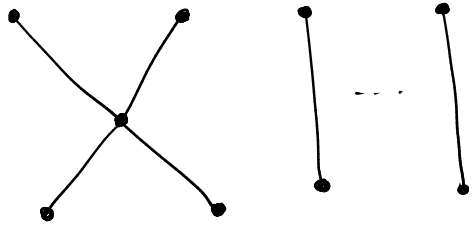
\includegraphics[width=0.2\textwidth]{feyn_a_n_1}
    \hspace{2cm}
    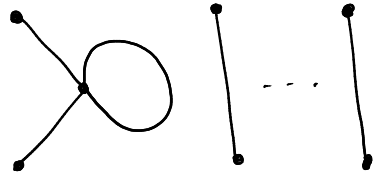
\includegraphics[width=0.2\textwidth]{feyn_a_n_2}
    \hspace{2cm}
    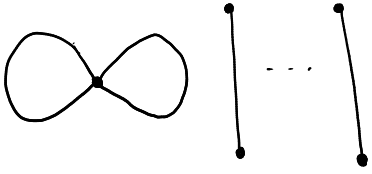
\includegraphics[width=0.2\textwidth]{feyn_a_n_3}
    \caption{Feynman diagrams for $a_n$}
    \label{fig:feyn_a_n}
  \end{figure}
  \begin{align}
    a_n = \frac{3}{4} \left( 2n^2 + 2n + 1 \right)
  \end{align}

  Note that $b_{n, m} \neq 0$ only if $\abs{n - m} \in \{2, 4\}$

  \begin{figure}[h]
    \centering
    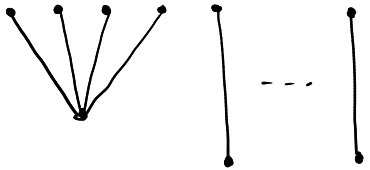
\includegraphics[width=0.2\textwidth]{feyn_b_nm_1}
    \caption{Feynman diagrams for $b_{n, m}$ for $\abs{n - m} = 4$}
    \label{fig:feyn_b_nm_1}
  \end{figure}

  \begin{align}
    b_{n, n-4} = \frac{1}{16} \sqrt{n(n-1)(n-2)(n-3)}
  \end{align}

  \begin{figure}[h]
    \centering
    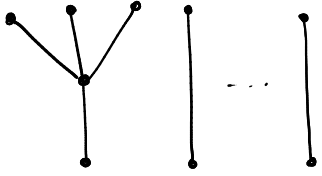
\includegraphics[width=0.2\textwidth]{feyn_b_nm_2}
    \hspace{2cm}
    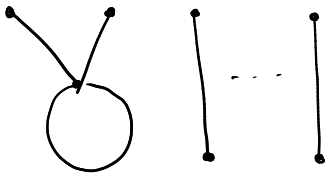
\includegraphics[width=0.2\textwidth]{feyn_b_nm_3}
    \caption{Feynman diagrams for $b_{n, m}$ for $\abs{n - m} = 2$}
    \label{fig:feyn_b_nm_2}
  \end{figure}

  \begin{align}
    b_{n, n-2} = \frac{(2n-1)}{4} \sqrt{n(n-1)} 
  \end{align}
  
  \begin{align}
    \ket{\alpha, t} &= e^{-i H t} \ket{\alpha} \\
    &= \sum_{n} \prescript{}{\lambda}{\braket{n}{\alpha}} e^{-i E_n t} \ket{n}_{\lambda} \\
    &= \ket{\alpha(t)} + \lambda \sum_{n} K_n e^{-i n t} \ket{n} \\
    K_n &= -i a_n t \braket{n}{\alpha}
  \end{align}

  Finally, we want to calculate the expectation values $\mel{\alpha, t}{a}{\alpha, t}$ and $\mel{\alpha, t}{a^2}{\alpha, t}$
  \begin{align}
    K_n = -\frac{3it}{4} e^{-\frac{1}{2} \abs{\alpha}^2} \frac{\alpha^n}{\sqrt{n!}} (2n^2 + 2n + 1)
  \end{align}

  


  \medskip

  \printbibliography[heading=bibintoc, title={References}]

\end{document}